\section{Theory}
\label{arithmetic}
The first step in finding a balanced arithmetic was finding a balancing scheme for individual values.
While the general shape of the scheme was pretty much clear from the start, the location of $x$ and $\bar{x}$ emerged during my work on the balanced operations.
\Cref{fig:schemes} shows the two schemes that are used in my project.

\begin{figure}[h]
  \centering
  \begin{subfigure}{.49\linewidth}
    \centering
    \tikzbox{scheme1.tex}
    \caption{Balancing Scheme 1}
    \label{fig:scheme1}
  \end{subfigure}
  \begin{subfigure}{0.49\linewidth}
    \centering
    \tikzbox{scheme2.tex}
    \caption{Balancing Scheme 2}
  \end{subfigure}
  \caption{Balancing Schemes}
  \label{fig:schemes}
\end{figure}

In my theoretical work I found balanced operations for both schemes, but in the end decided to use Scheme 1 because it exhibits nicer behavior for shifts, especially rotations.
Both are worth mentioning however, because many of my operations will result in values formatted in Scheme 2 and require explicit transformation.
By finding standardized transformations in both directions I could reuse them in the rest of my arithmetic.

The biggest problem of finding a balanced arithmetic was that $\neg{x \circ y}$ is not $\neg{x} \circ \neg{y}$ ($\circ$ here denotes any operator).
As the ALU cannot execute two different operations on parts of the same register at the same time, there \emph{must} be imbalanced temporary values during execution.
My goal then was to limit the number of these imbalanced values.

\subsection{Finding Balanced Operations}
\label{operations}
After fixing the balancing scheme I started working on finding balanced variants for \ir{}'s binary operators.
As stated above, most operations do not preserve balancedness over all intermediate steps.
They do, however, decrease the signal-to-noise ration for an attacker.
A more detailed analysis can be found in \Cref{balance-eval}.

The notation for the rest of this section is the following:
A single line denotes an intermediate 32bit value, with the individual bytes split by $\bsep{}$.
Notes to the right of $|$ explain how the value in the current line was derived.

\subsubsection{Scheme 1 to Scheme 2}
The transformation from Scheme 1 to Scheme 2 looks as follows:
\begin{align*}
  \binp{1}{0}{\neg{x}}{0}{x}\\
  \btrans{2}{\neg{x}}{\neg{x}}{x}{x}{\%1 \blsl 8}\\
  \btrans{3}{\neg{x}}{0}{0}{x}{\%2 \band \hex{ff0000ff}}
\end{align*}

LSL here stands for logical shift left.

\subsubsection{Scheme 2 to Scheme 1}
The other direction works very similar to the first, and is shown below.
Note that ROR stands for rotational right shift, i.e. the values shifted out on the right are shifted back in on the left.
\begin{align*}
  \binp{1}{\neg{x}}{0}{0}{x}\\
  \btrans{2}{\hex{ff}}{\neg{x}}{0}{x}{\%1 \borr (\%1 \bror 24)}\\
  \btrans{3}{0}{\neg{x}}{0}{x}{\%2 \band \hex{00ff00ff}}
\end{align*}

\subsubsection{ORR}
Before finding a balanced variant of bitwise OR, I needed to find an expression for the inverse of the result.
For this I utilized DeMorgan's law: $\neg{x \lor y} = \neg{x} \land \neg{y}$.
With this equality ORR looks as follows:
\begin{align*}
  \binp{1}{0}{\neg{x}}{0}{x}\\
  \binp{2}{0}{\neg{y}}{0}{y}\\
  \btrans{3}{0}{\neg{x} \borr \neg{y}}{0}{x \borr y}{\%1 \borr \%2}\\
  \btrans{4}{0}{\neg{x} \band \neg{y}}{0}{x \band y}{\%1 \band \%2}\\
  \btrans{5}{\neg{x} \band \neg{y}}{\neg{x} \borr \neg{y}}{x \band y}{x \borr y}{\%3 \borr (\%4 \blsl 8)}\\
  \btrans{6}{\neg{x \borr y}}{0}{0}{x \borr y}{\%5 \band \hex{ff0000ff}}\\
  \btrans{7}{0}{\neg{x \borr y}}{0}{x \borr y}{\trans21(\%6)}
\end{align*}

\subsubsection{AND}
As $\neg{x \land y} = \neg{x} \lor \neg{y}$, AND works almost the same as ORR, but uses different parts of the intermediate results.

\subsubsection{XOR}
XOR is at its base a combination of AND and ORR: $x \oplus y = (\neg{x} \land y) \lor (x \land \neg{y})$.
It is better to create a balanced XOR from scratch, instead of compositioning it from ORR and AND, because both ORR and AND have the same imbalanced intermediate values.

The inverse of the result can be found through repeated application of DeMorgan's law and simplification.
I will skip the details of this simple transformation, and show only the result: $\neg{x \oplus y} = (x \land y) \lor (\neg{x} \land \neg{y})$.

\begin{align*}
  \binp{1}{0}{\neg{x}}{0}{x}\\
  \binp{2}{0}{\neg{y}}{0}{y}\\
  \btrans{3}{\neg{x}}{\neg{x}}{x}{x}{\%1 \borr (\%1 \blsl 8)}\\
  \btrans{4}{y}{\neg{y}}{\neg{y}}{y}{\%2 \borr (\%2 \bror 24)}\\
  \btrans{5}{\neg{x} \band y}{\neg{x} \band \neg{y}}{x \band \neg{y}}{x \band y}{\%3 \band \%4}\\
  \btrans{6}{x \bxor y}{\neg{x \bxor y}}{x \bxor y}{\neg{x \bxor y}}{\%5 \band (\%5 \bror 16)}\\
  \btrans{7}{\neg{x \bxor y}}{x \bxor y}{\neg{x \bxor y}}{x \bxor y}{\%6 \bror 8}\\
  \btrans{8}{\neg{x \bxor y}}{0}{0}{x \bxor y}{\%7 \band \hex{ff0000ff}}\\
  \btrans{9}{0}{\neg{x \bxor y}}{0}{x \bxor y}{\trans21 (\%8)}
\end{align*}

\subsubsection{ADD}
For the inverse of arithmetic operations I utilized the definition of the negation in 2s complement: $-x = \neg{x} + 1$.
This also means that $\neg{x} = -x - 1$ and therefore:
\begin{equation*}
  \neg{x + y} = - (x + y) - 1 = - x - y - 1 = \neg{x} + 1 + \neg{y} \cancel{+ 1} \cancel{- 1} = \neg{x} + \neg{y} + 1
\end{equation*}

Using associativity of addition the balanced variant of ADD looks like the following:
\begin{align*}
  \%1 &= 0 && \bsep \neg{x} &&\bsep 0 &&\bsep x      &&\\
  \%2 &= 0 && \bsep \neg{y} &&\bsep 0 &&\bsep y      &&\\
  \%3 &= 0 && \bsep \neg{x}+1 &&\bsep 0 &&\bsep x    &&\;|\ \%1 + \hex{00010000}\\
  \%4 &= c && \bsep \neg{x+y} &&\bsep c' &&\bsep x+y &&\;|\ \%3 + \%2\\
  \%5 &= 0 && \bsep \neg{x+y} &&\bsep 0 &&\bsep x+y  &&\;|\ \%4 \land \hex{00ff00ff}
\end{align*}
Both $c$ and $c'$ denote possible carry values that need to be filtered.

\subsubsection{SUB}
For subtraction I again use the definition of 2s complement, giving me the following for the inverse result:
\begin{equation*}
  \neg{x-y} = - (x-y) - 1 = y - x - 1 = y + (-x -1) = y + \neg{x} = \neg{x} + y
\end{equation*}
Applying the same definition to the regular result yields
\begin{equation*}
  x-y = x + \neg{y} + 1
\end{equation*}
resulting in a quick and convenient balanced subtraction:
\begin{align*}
  \binp{1}{0}{\neg{x}}{0}{x}\\
  \binp{2}{0}{\neg{y}}{0}{y}\\
  \btrans{3}{0}{y}{0}{\neg{y}}{\%2 \bror 16}\\
  \btrans{4}{0}{y}{c}{\neg{y}+1}{\%3 + \hex{00000001}}\\
  \btrans{5}{c'}{\neg{x}+y}{c''}{x+\neg{y}+1}{\%1 + \%4}\\
  \btrans{6}{0}{\neg{x-y}}{0}{x-y}{\%5 \band \hex{00ff00ff}}
\end{align*}

\subsubsection{MUL}
The inverse result of multiplication can be calculated as follows:
\begin{equation*}
  \neg{x \cdot y} = -(x \cdot y) - 1 = (-x) \cdot y - 1 = (\neg{x} + 1) \cdot y = \neg{x} \cdot y + y - 1
\end{equation*}

Which gives us the following balanced multiplication:
\begin{align*}
  \binp{1}{0}{\neg{x}}{0}{x}\\
  \binp{2}{0}{\neg{y}}{0}{y}\\
  \btrans{3}{\neg{y}}{0}{0}{y}{\trans21(\%2)}\\
  \btrans{4}{c}{\neg{x}\cdot y}{c'}{x \cdot y}{\%1 \cdot \%3}\\
  \btrans{5}{c''}{\neg{x \cdot y} +1}{c'}{x \cdot y}{\%4 + (\%2 \blsl 16)}\\
  \btrans{6}{c'''}{\neg{x \cdot y}}{c'}{x \cdot y}{\%5 + \hex{00ff0000}}\\
  \btrans{7}{0}{\neg{x \cdot y}}{0}{x \cdot y}{\%6 \band \hex{00ff00ff}}
\end{align*}

\subsubsection{DIV and REM}
I used repeated balanced subtraction for DIV and REM operations.
The code was written in C and can be found in the git of my thesis\cite{git}.
%TODO: include?

\subsubsection{Shifting}
While performing logical shifts, I need to ensure that the correct bits are pushed in.
When 0s are shifted in for $x$ I have to shift in 1s for $\neg{x}$, and vice versa.
This is done by ORRing the target value with \hex{ff000000} or \hex{0000ff00}, as needed.
The shifting is performed normally and the result is then AND filtered with \hex{00ff00ff} to comply with Scheme 1 again.

\subsection{Testing for Correctness}
Before I started implementing my balancing pass I wanted to verify the correctness of my arithmetic.
For this purpose I wrote python code to calculate all operations step by step while saving the intermediate results.
\Cref{lst:multiop} shows the intermediate steps for multiplication.

\begin{lstlisting}[language=python, caption=Step-by-step execution of balanced multiplication, label=lst:multiop]
m = MultiStepOperation([
    Convert_1_2(1), #2
    BinaryOperation(0,2, lambda x,y: (x*y) & 0xffffffff), #3 the AND is required due to python's arbitrary precision integers
    BinaryOperation(3,1, lambda x,y: x + (y << 16)), #4
    UnaryOperation(4, lambda x: x + 0x00ff0000), #5
    UnaryOperation(5, lambda x: x & 0x00ff00ff), #6
])
\end{lstlisting}

The \emph{Unary-} and \emph{BinaryOperation} classes take the indices of the layers to operate on (0 and 1 are the inputs, all others are intermediate values), as well as the operation in form of a lambda.
Executing the \emph{MultiStepOperation} will then execute all lambdas in order and store the intermediate results in \emph{numpy} arrays.
Correctness is then tested by checking if all final results are equal to the output of a function to compare to ($x \cdot y$ in this case).

%% \begin{lstlisting}[language=python, caption=Testing correctness of balanced operation, label=lst:correctness]
%% def unbalanceScheme1(x):
%%     return x & word_filter

%% vUS1 = np.vectorize(unbalanceScheme1)


%% def testCorrectness(self, equivalentUnbalancedFunction):
%%     uResults = vUS1(self.results[-1])
%%     incorrectResults = {}
%%     for i in range(word_max):
%%         for j in range(word_max):
%%             r = equivalentUnbalancedFunction(i, j)
%%             r &= word_filter
%%             if r != uResults[i*word_max + j]:
%%                 incorrectResults[(i,j)] = (r, uResults[i*word_max + j])
%%     return incorrectResults
%% \end{lstlisting}

\subsection{Evaluating the Balancedness}
\label{balance-eval}
Balancedness of my operations is evaluated using the same python code.
As all intermediate results are stored during evaluation I can easily calculate the distribution of their \hammingw s, as shown in \Cref{fig:mult}.
I used these histograms to check if operations needed improvement, and if that was the case, I tried to find a different, more balanced way of performing them.

\begin{figure}[h]
  \centering
  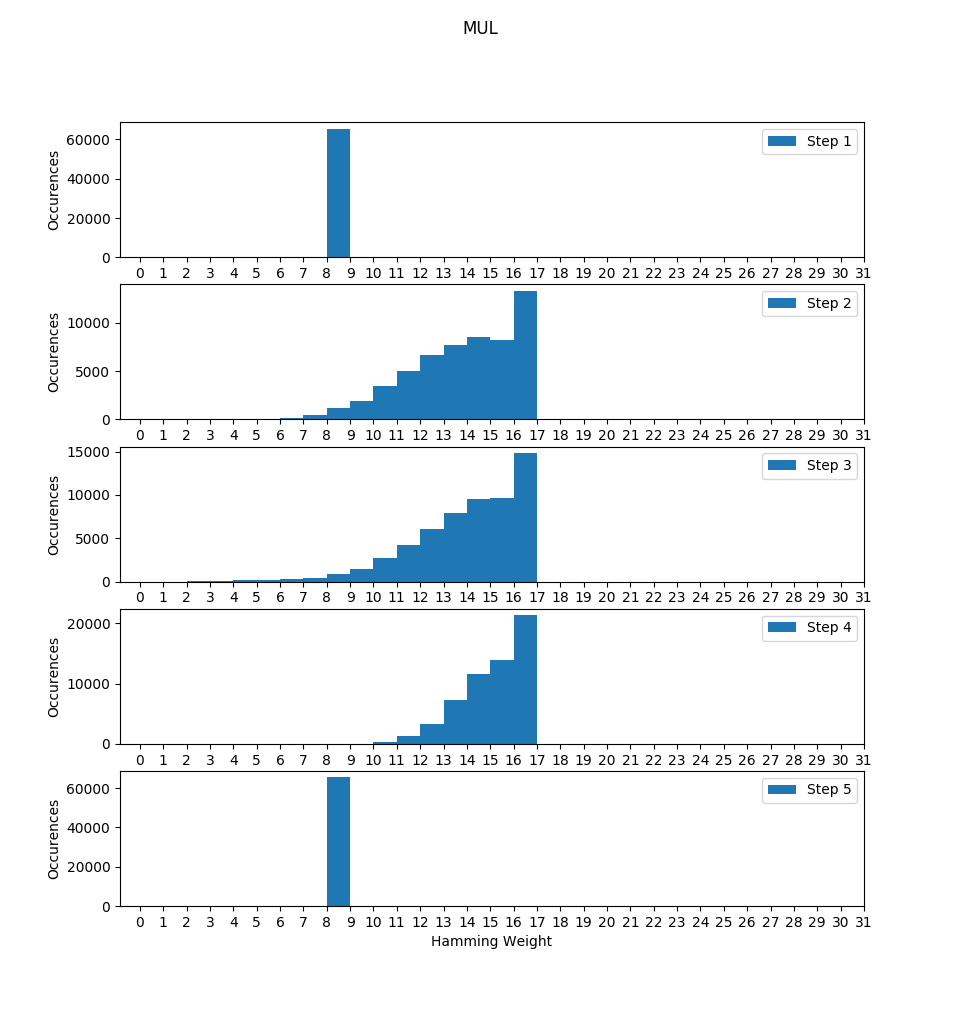
\includegraphics[width=\textwidth]{multiplication.png}
  \caption{Histogram of \hammingw s of direct balanced multiplication}
  \label{fig:mult}
\end{figure}

While \Cref{fig:mult} shows imbalanced values in the intermediate steps, it performed faster and better than multiplication via repeated addition.
\Cref{fig:mult-comparison} shows an evaluation of both variants, evaluated over the multiplications of all possible 8bit factors.

\begin{figure}[hp]
  \centering
  \begin{subfigure}[b]{0.49\textwidth}
    \begin{tikzpicture}
\begin{axis}[
    ybar,
    bar width=0.015\textwidth,
    enlargelimits=0.05,
    xtick={0,8,16,24,32},
    width=\textwidth
]
\addplot[pantone289,fill=pantone289!40] table [x=i, y=loop-total, col sep=comma] {data/multiplication.csv};
\end{axis}
\end{tikzpicture}

    \caption{Addition-loop multiplication}
  \end{subfigure}
  \begin{subfigure}[b]{0.49\textwidth}
    \begin{tikzpicture}
\begin{axis}[
    ybar,
    bar width=0.015\textwidth,
    enlargelimits=0.05,
    xtick={0,8,16,24,32},
    width=\textwidth,
]
\addplot[pantone289,fill=pantone289!40] table [x=i, y=direct-total, col sep=comma] {data/multiplication.csv};
\end{axis}
\end{tikzpicture}

    \caption{Direct multiplication}
  \end{subfigure}

  \begin{subfigure}[b]{\textwidth}
    % This file was created by matplotlib2tikz v0.7.4.
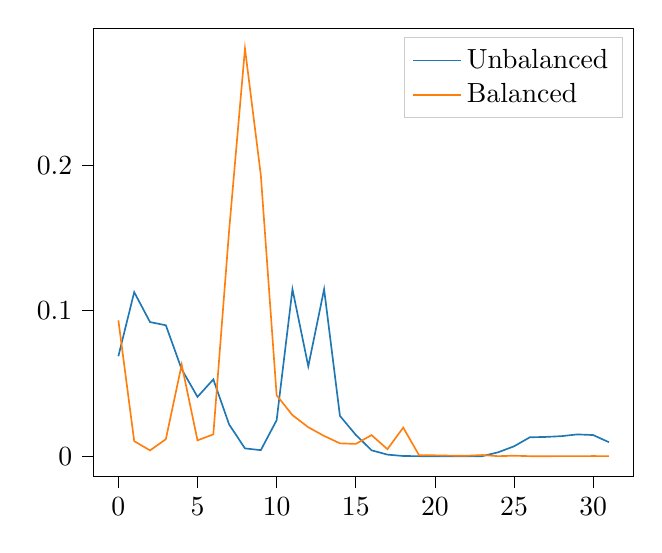
\begin{tikzpicture}

\definecolor{color0}{rgb}{0.12156862745098,0.466666666666667,0.705882352941177}
\definecolor{color1}{rgb}{1,0.498039215686275,0.0549019607843137}

\begin{axis}[
legend cell align={left},
legend style={draw=white!80.0!black},
tick align=outside,
tick pos=left,
x grid style={white!69.01960784313725!black},
xmin=-1.55, xmax=32.55,
xtick style={color=black},
y grid style={white!69.01960784313725!black},
ymin=-0.0140054362142874, ymax=0.294114160500036,
ytick style={color=black}
]
\addplot [semithick, color0]
table {%
0 0.0686886708296164
1 0.112735781975203
2 0.0921666731308743
3 0.0899559141036083
4 0.0597292789822751
5 0.0407632936430982
6 0.0527737915163738
7 0.0217455946424647
8 0.0053394355453852
9 0.00412416450115709
10 0.0247062017608502
11 0.114713829525915
12 0.0617719686098075
13 0.114752614772007
14 0.0276926657099639
15 0.014647894607558
16 0.00403366559360819
17 0.00106013005985856
18 0.000116355738277159
19 0
20 0
21 0
22 0
23 0
24 0.00268911039573879
25 0.0067744896508035
26 0.0129801290255853
27 0.0132257689175038
28 0.0137558339474331
29 0.014958176576297
30 0.0145186104539167
31 0.00957995578481946
};
\addlegendentry{Unbalanced}
\addplot [semithick, color1]
table {%
0 0.0933479074509321
1 0.0103489919568661
2 0.00395656502417046
3 0.0116729786964718
4 0.0629030547487333
5 0.0108672968433009
6 0.0149863666998519
7 0.155431595729031
8 0.280108724285749
9 0.193293511096514
10 0.041845849626581
11 0.0281903119750666
12 0.0198957232149272
13 0.0138984396114937
14 0.00882315710967195
15 0.00843143493477569
16 0.0144680618134171
17 0.00481014303846404
18 0.0196511106777649
19 0.000639755866424449
20 0.000585017396569951
21 0.000352378899688333
22 0.000290798121102022
23 0.000780023195426601
24 0
25 0.0003061933157486
26 0
27 0
28 3.42115436590614e-06
29 1.36846174636246e-05
30 7.0133664501076e-05
31 2.73692349272492e-05
};
\addlegendentry{Balanced}
\end{axis}

\end{tikzpicture}
    \caption{Scaled Hamming weight histograms for multiplication variants}
  \end{subfigure}
  \caption{Hamming weight histograms for direct and addition-loop multiplication}
  \label{fig:mult-comparison}
\end{figure}

